%% Template article for Elsevier's document class `elsarticle`
\documentclass[preprint,12pt, a4paper]{elsarticle}

\usepackage{graphicx}
\usepackage{hyperref}
\usepackage{orcidlink}
\usepackage{caption}

\journal{SoftwareX}

\begin{document}

\begin{frontmatter}

\title{Graphical Abstract: A Modular NLU-Solr Architecture with Dynamic GIS Visual Synchronization for Conversational Spatial Search}

\author[1]{F{\'e}lix de Miguel \orcidlink{0009-0000-9607-110X}\corref{cor1}}
\ead{fdemiguel@ubu.es}

\author[1]{Daniel Urda \orcidlink{0000-0003-2662-798X}}
\ead{durda@ubu.es}

\author[1]{Nu{\~n}o Basurto \orcidlink{0000-0001-7289-4689}}
\ead{nbasurto@ubu.es}

\cortext[cor1]{Corresponding author at: Grupo de Inteligencia Computacional Aplicada (GICAP), Departamento de Digitalizaci{\'o}n, Escuela Polit{\'e}cnica Superior, Universidad de Burgos, Av. Cantabria s/n, 09006 Burgos, Spain.}

\address[1]{Grupo de Inteligencia Computacional Aplicada (GICAP), Departamento de Digitalizaci{\'o}n, Escuela Polit{\'e}cnica Superior, Universidad de Burgos, Av. Cantabria s/n, 09006 Burgos, Spain}

\end{frontmatter}

\section*{Graphical Abstract}

\begin{figure}[h!]
\centering
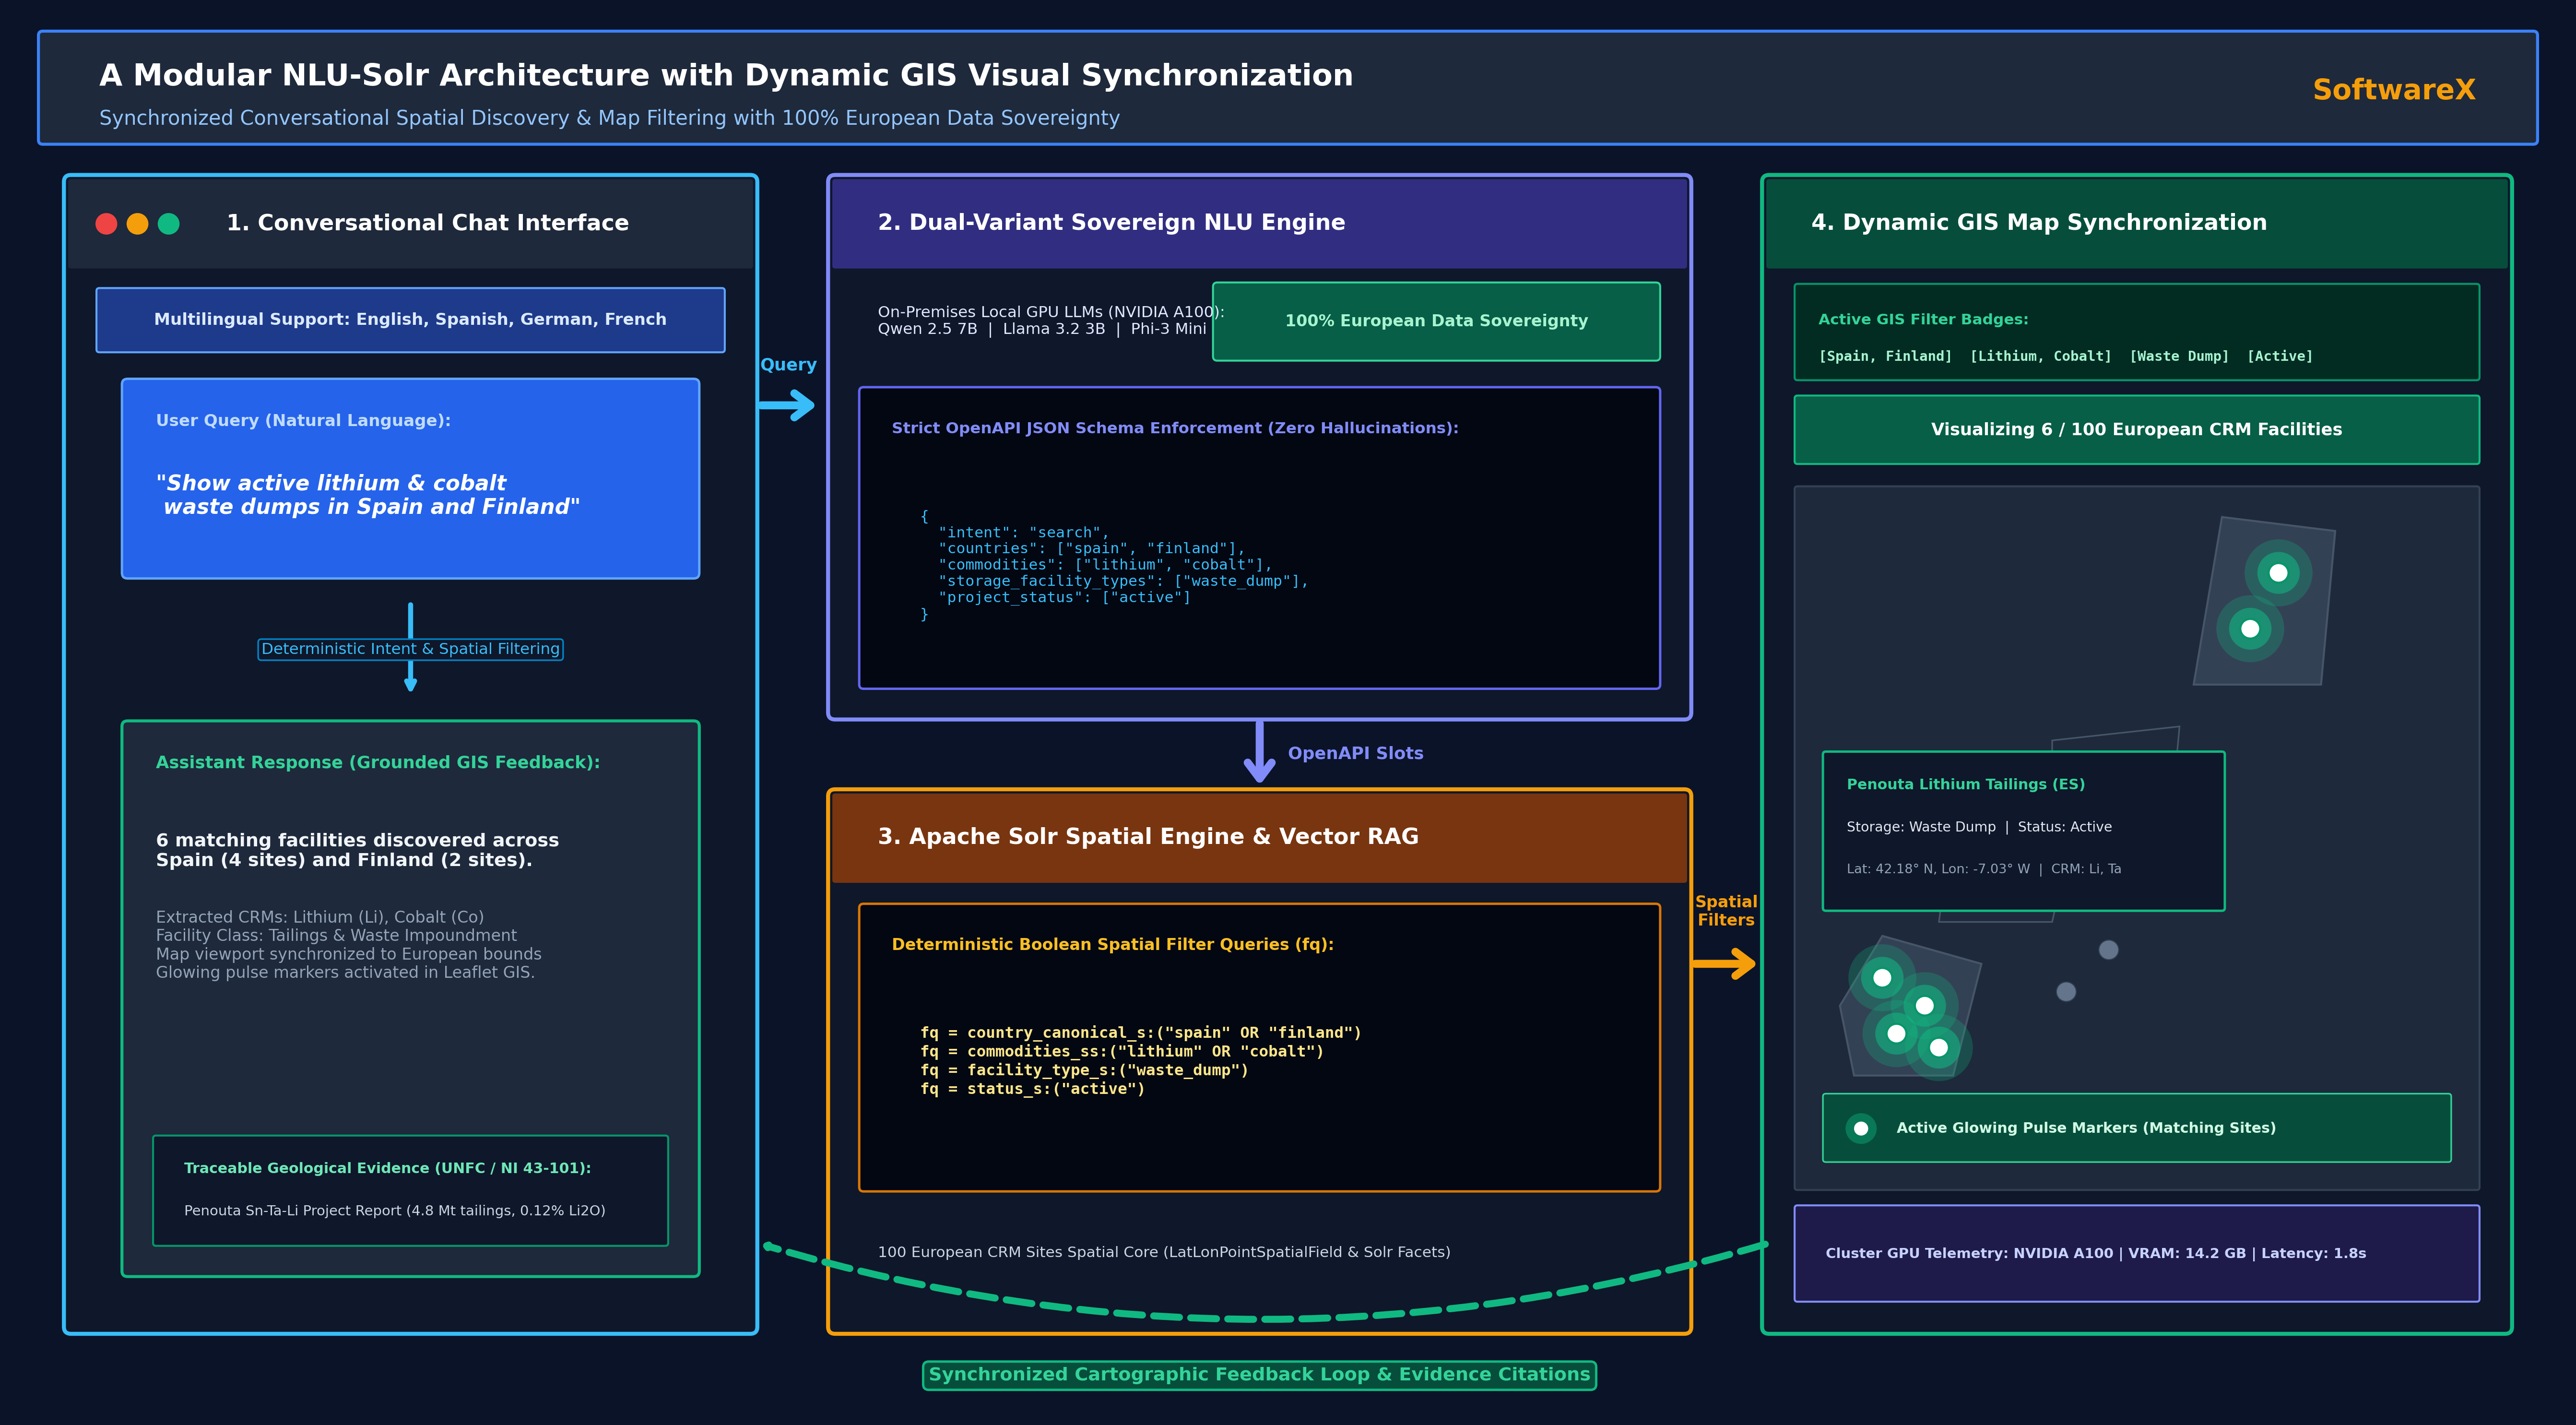
\includegraphics[width=\textwidth]{graphical_abstract.png}
\caption*{Graphical Abstract: Decoupled 4-stage software architecture combining Few-Shot NLU intent parsing, pluggable domain thesaurus normalization, Apache Solr spatial indexing, and dynamic Leaflet.js GIS visual synchronization.}
\end{figure}

\end{document}
